% !TeX root = main.tex

\hypertarget{limits-of-functions}{%
\section{Limits of Functions}\label{limits-of-functions}}

\hypertarget{intuitive-definition}{%
\subsection{Intuitive definition}\label{intuitive-definition}}

\noindent\textbf{Limits:}

We say that the limit of \(f(x)\) as \(x\) approaches \(a\) is \(L\) if $f(x)$ can get arbitrarily close to $L$ when \(x\) approaches to \(a\). 

\[\lim\limits_{x \to a} f(x)=L\]

\noindent\textbf{Limit from the left:}

We say that \(L\) is the left limit of \(f(x)\) if $f(x)$ can get arbitrarily close to $L$ when \(x\) approaches to \(a\) from the left.

\[\lim\limits_{x \to a^{-} }f(x)=L.\]

\textbf{Limit from the right:}

We say that \(L\) is the right limit of \(f(x)\) if $f(x)$ can get arbitrarily close to $L$ when \(x\) approaches to \(a\) from the right.

\[\lim\limits_{x \to a^+}f(x)=L.\]

\hypertarget{determine-limits-from-graphs}{%
\subsection{Determine limits from
graphs}\label{determine-limits-from-graphs}}

\begin{example}
  Using the graph of the function \(f\) shown below to
  determine the limit \(\lim\limits_{x\to -4}f(x)\) and the limit
  \(\lim\limits_{x\to 2} f(x)\).
  
  \begin{figure}[h]
    \centering
  \href{https://www.geogebra.org/m/Ktr9uqYu}{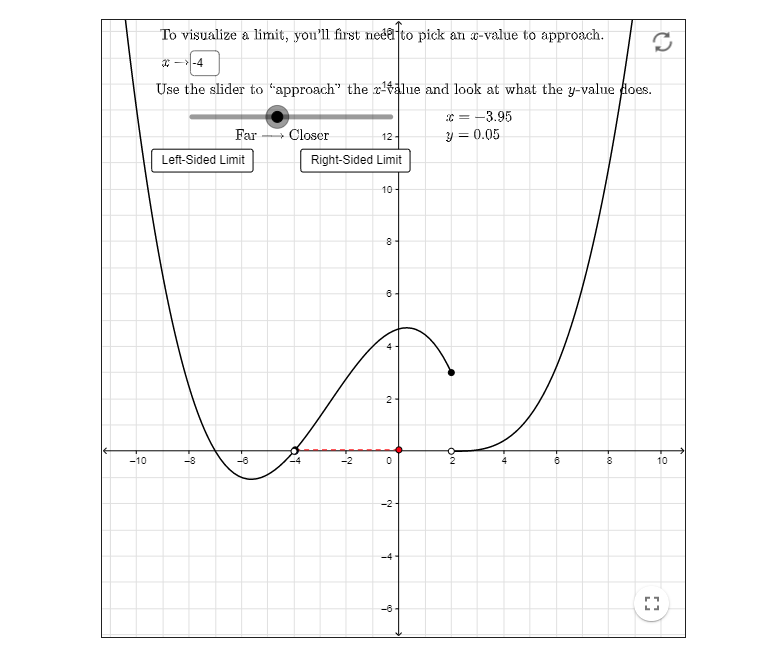
\includegraphics[height=0.3\textheight]{img/clip_image001.png}}
  \end{figure}
\end{example}
\vspace*{2\baselineskip}

\begin{example}
  Using the graph of the function \(g\) to evaluate the
  limit \(\lim\limits_{x\to -1}g(x)\).
  
  \begin{figure}[h]
  \centering
  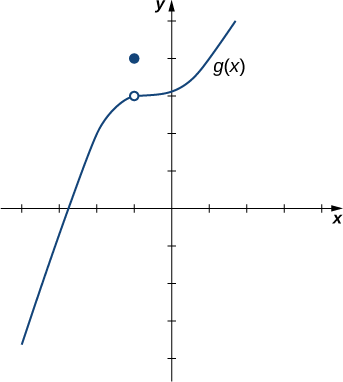
\includegraphics[scale=0.8]{img/imageedit_9_2225331012.png}
  \end{figure}
\end{example}
\vspace*{2\baselineskip}

\hypertarget{determine-limits-numerically-using-tables}{%
\subsection{Determine limits numerically using
tables}\label{determine-limits-numerically-using-tables}}

Numerically, we say that
\(\lim\limits_{x\to a}f(x)=L\) if for any \(\varepsilon>0\) there exists
a number \(\delta>0\) such that \(|f(x)-L|<\varepsilon\) whenever
\(|x-a|<\delta\).

\begin{example}
  Use a table to determine the limit
  \(\lim\limits_{x\to 1}x\).
\end{example}
\vspace*{6\baselineskip}

\begin{example}
  Use a table to determine the limit
  \(\lim\limits_{x\to 1}c\), where \(c\) is a constant number.
\end{example}
\vspace*{6\baselineskip}

\begin{example}
  Use a table to determine the limit
  \(\lim\limits_{x\to 0}\dfrac{\sin x}{x}\).
\end{example}
\vspace*{6\baselineskip}

\begin{example}
  Use a table to determine the limit
  \(\lim\limits_{x\to 0}\sin\left(\frac1x\right)\).
\end{example}
\vspace*{6\baselineskip}

\subsection{One-sided limits}

\begin{example}
  For the function
  \(f(x)=\begin{cases}x+1, & \text{if }x<2\\ x^2-4, & \text{if }x\ge 2\end{cases}\),
  determine each of the following limits.
  
  \begin{enumerate}
  \item
    \(\lim\limits_{x \to 2^-}f(x)\)
  \item
    \(\lim\limits_{x \to 2^+}f(x)\)
  \item
    \(\lim\limits_{x\to 2}f(x)\)
  \end{enumerate}
\end{example}

\begin{example}
  For the function
  \(f(x)=\begin{cases}x^2+1, & \text{if }x<1\\ 3x-1, & \text{if }x\ge 1\end{cases}\),
  determine each of the following limits.
  
  \begin{enumerate}
  \item
    \(\lim\limits_{x \to 1^-}f(x)\)
  \item
    \(\lim\limits_{x \to 1^+}f(x)\)
  \item
    \(\lim\limits_{x\to 1}f(x)\)
  \end{enumerate}
\end{example}

\begin{theorem}
  Let \(f(x)\) be a function defined at all values in an
  open interval containing \(a\), with the possible exception of \(a\)
  itself, and let \(L\) be a real number. Then,
  \[\lim\limits_{x \to a}f(x)=L\]
  if and only if \(\lim\limits_{x \to a^-}f(x)=L\) and
  \(\lim\limits_{x \to a^+} f(x)=L\).
\end{theorem}

\hypertarget{infinite-limits}{%
\subsection{Infinite limits}\label{infinite-limits}}

\textbf{Infinite limits from the left:} Let \(f(x)\) be a function
defined at all values in an open interval of the form \((b,a)\).

\begin{enumerate}[sepno]
\item
  If the values of \(f(x)\) can be arbitrarily large as the values of
  \(x\) (where \(x<a\)) approach the number \(a\), then we say that the
  limit as \(x\) approaches \(a\) from the left is positive infinity and
  we write \[\lim\limits_{x \to a^-}f(x)=+\infty.\]
\item
  If the values of \(f(x)\) can be arbitrarily large as the values of
  \(x\) (where \(x<a\)) approach the number \(a\), then we say that the
  limit as \(x\) approaches \(a\) from the left is negative infinity and
  we write \[\lim\limits_{x \to a^-}f(x)=-\infty.\]
\end{enumerate}

\textbf{Infinite limits from the right:} Let \(f(x)\) be a function
defined at all values in an open interval of the form \((a,c)\).

\begin{enumerate}[sepno]
\item
  If the values of \(f(x)\) can be arbitrarily large as the values of
  \(x\) (where \(x>a\)) approach the number \(a\), then we say that the
  limit as \(x\) approaches \(a\) from the left is positive infinity and
  we write \[\lim\limits_{x \to a^+}f(x)=+\infty.\]
\item
  If the values of \(-f(x)\) can be arbitrarily large as the values of
  \(x\) (where \(x>a\)) approach the number \(a\), then we say that the
  limit as \(x\) approaches \(a\) from the left is negative infinity and
  we write \[\lim\limits_{x \to a^+}f(x)=-\infty.\]
\end{enumerate}

\textbf{Two-sided infinite limit:} Let \(f(x)\) be defined for all
\(x\neq a\) in an open interval containing \(a\)

\begin{enumerate}[parsep=0pt,after=\vspace{0pt}]
\item
  If the values of \(f(x)\) can be arbitrarily large as the values of
  \(x\) (where \(x\neq a\)) approach the number \(a\), then we say that the
  limit as \(x\) approaches \(a\) is positive infinity and we write
  \[\lim\limits_{x \to a} f(x)=+\infty.\]
\item
  If the values of \(-f(x)\) can be arbitrarily large as the values of
  \(x\) (where \(x\neq a\)) approach the number \(a\), then we say that the
  limit as \(x\) approaches \(a\) is negative infinity and we write
  \[\lim\limits_{x \to a}f(x)=-\infty.\]
\end{enumerate}

\begin{example}
  Evaluate each of the following limits, if possible.
  
  \begin{enumerate}
  \item
    \(\lim\limits_{x \to 0^-} \frac{1}{x}\)
  \item
    \(\lim\limits_{x \to 0^+} \frac{1}{x}\)
  \item
    \(\lim\limits_{x \to 0}\frac{1}{x}\)
  \end{enumerate}
\end{example}

\subsection{Practice}


\begin{exercise}
  Use the graph of \(h(x)\) shown below to determine
  the limit \(\lim\limits_{x \to 2}h(x)\).
  
  \begin{figure}[h!]
  \centering
  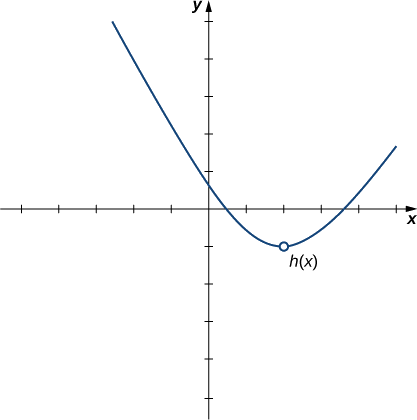
\includegraphics[scale=0.8]{img/imageedit_13_2727890618.png}
  \end{figure}
\end{exercise}
\vspace*{\baselineskip}


\begin{exercise}
  Determine the limit
  \(\lim\limits_{x\to 1}\dfrac{\frac1x-1}{x-1}\).
\end{exercise}
\vspace*{6\baselineskip}

\begin{exercise}
  Determine the limit
  \(\lim\limits_{x\to 0}x\sin\left(\frac1x\right)\).
\end{exercise}
\vspace*{6\baselineskip}

\begin{exercise}
  Determine the limits
  
  \begin{enumerate}
  \item
    \(\lim\limits_{x\to 1^-}\dfrac{|x-1|}{x-1}\).
  \item
    \(\lim\limits_{x\to 1^+}\dfrac{|x-1|}{x-1}\).
  \item
    \(\lim\limits_{x\to 1^+}\dfrac{|x-1|}{x-1}\).
  \end{enumerate}
\end{exercise}

\begin{exercise}
  Evaluate each of the following limits, if possible.
  
  \begin{enumerate}
  \item
    \(\lim\limits_{x \to 0^-}\frac{1}{x^2}\)
  \item
    \(\lim\limits_{x \to 0^+}\frac{1}{x^2}\)
  \item
    \(\lim\limits_{x \to 0}\frac{1}{x^2}\)
  \end{enumerate}
\end{exercise}
